\section{Realisierung}
Wie bereits in der Systembeschreibung beschrieben, wird der Fahrsimulator in drei Hauptkomponenten unterteilt: den UDP-Listener, den Szenen-Manager und das Hauptprogramm. Da die Verbindung zwischen dem Cockpit und dem Fahrsimulator mit einer Netzwerkschnittstelle realisiert wird, ist es möglich, die Anbindung an das Cockpit und den Fahrsimulator physisch auf zwei unterschiedlichen Rechnern zu betreiben. Eine Alternative ist die Umsetzung mit dem \gls{ogre}-Framwork (siehe Anhang \ref{ogre-framework}). Dieses Framework bietet umfassende Lösungen, um Steuerradär und Pedalen, wie sie in userem Cockpit vorhanden sind, anzusteuern.\\
Da die 3D-Umgebung mit fortscheitendem Projekt ausgebaut wird, könnte sich die notwendige Rechenleistung erheblich steigern. Folgen ungenügender Leistung sind unregelmässige Bewegungen (Lags) in der virtuellen Umgebung oder sogar der Absturz des gesamten Programms.\\
Aus diesem Grund ist die erste Variante mit der Netzwerkschnittstelle für das Fahrsimulatorprojekt besser geeignet. Die andere Variante wird verworfen.

\subsection{LabVIEW Programm}
Eine LabVIEW-Umgebung existiert bereits auf dem Rechner, an den das Cockpit angeschlossen ist. Ein LabVIEW-Programm liest bereits die Eingaben im Cockpit ein. Da dieses Programm jedoch nicht genau den Anforderungen entspricht, wird es neu realisiert. Die Eingaben werden über einen UDP-Socket alle 10 ms gesendet. Zusätzlich wird ein zweiter UDP-Socket eingerichtet, um Packete, die vom Fahrsimulator zurück gesendet werden, zu empfangen. Die Daten der empfangenen Packete werden von LabVIEW verarbeitet, dargestellt und in ein Log-File geschrieben.\\
Das detaillierte LabVIEW Programm ist im Anhang \ref{labview_programme} zu finden. Die LabVIEW-Schnittstelle ist im Anhang \ref{labview_schnittstelle} genauer ausgeführt.

\subsection{UDP-Listener}
\label{sec:udp-listener}
In einem eigenen Thread werden UDP-Pakete kontinuierlich gelesen und verarbeitet. Die Informationen werden zwischengespeichert, so dass sie bei jedem Renderdurchlauf zur Verfügung stehen. Dank der Häufigkeit, mit der Pakete versendet werden, stellt das Verlieren eines Pakets kein Problem dar, wodurch UDP sich durch den Geschwindigkeitsvorteil gegenüber TCP besser eignet.

\begin{figure}[H]
\centering 
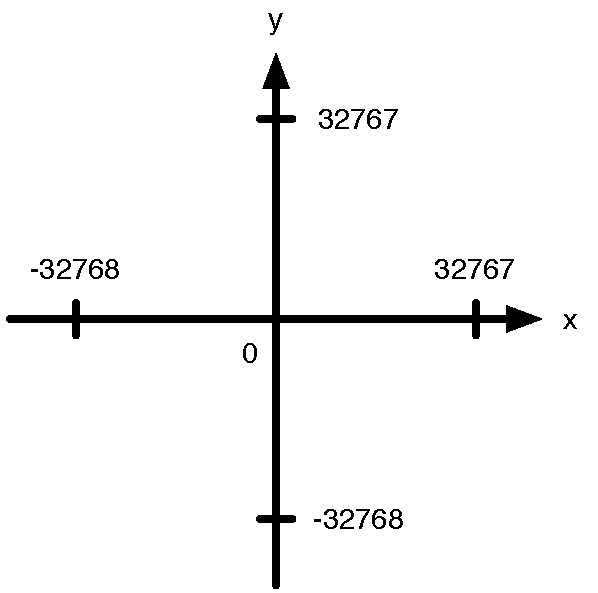
\includegraphics[width=0.5\linewidth]{src/koordinatensystem.pdf}
\caption{Koordinatensystem der Joystickeingabe} % Titel der Grafik
\label{Koordinatensystem} % Labelname
\end{figure}

Die von LabVIEW empfangenen Daten sind in erster Linie Parameter, die den Ausschlag der Pedalen und den Einschlagwinkel des Steuerrades representieren. Die beiden Pedalen werden in einem Koordinatensystem wie in Abbildung \ref{Koordinatensystem} auf der y-Achse im Bereich von -32768 bis 32767 abgebildet. Dabei heisst ein negativer y-Wert, dass das Gaspedal gedrückt wird, ein positiver Wert steht für das Drücken der Bremse. Der x-Wert im Koordinatensystem quantifiziert den Einschlagswinkel des Steuerrades. Hier steht -32768 einem vollständig nach links eingeschlagenen Steuerrad, 32767 einer Drehung bis zum rechten Anschlag. Sollte es zu einem späteren Zeitpunkt nötig sein, Tastendrücke am Steuerrad zu übermitteln, kann das UDP-Paket einfach erweitert werden.\\
Nebst den Eingaben durch Steuerrad und Pedalen wird von LabVIEW ein Timestamp gesendet. Der Timestamp wird von UDP-Listener empfangen und nach dem Abspeichern der Parameter wieder zurückgeschickt. Somit kann festgestellt werden, wieviel Verzögerung durch Kommunikation und Verarbeitung der Daten verursacht wird.\\

\subsection{Virtual Reality}
Eine erste Idee, um eine virtuelle Realität zu erzeugen, war der Einsatz von google Street View oder google Maps. Google Maps bietet die Möglichkeit, da die Satellitenbilder von der ganzen Erde gemacht wurden, überall auf der Welt zu fahren. Jedoch ist die Auflösung der Bilder nicht immer hoch genug, um damit eine Umgebung für der Fahrer generieren zu können. Erschwerend kommt hinzu, dass die Aufnahmen nur von oben gemacht wurden und somit keine Seitenansicht einer steilen Felswand oder eines Hauses zur Verfügung steht. Auch werden, da die Fotos aus der Vogelperspektive gemacht wurden, verschiedene Elemente die sich über der Strasse befinden zweidimensional angezeigt, wie zum Beispiel Bäume, Brücken oder Autos. Dies bedeutet, dass keine klare Strasse sichtbar ist. Somit würde der Einsatz von google maps zu keiner zufriedenstellenden Lösung führen. \\
Eine bessere Auflösung und Darstellung der Strassen bietet Google Street View. Hier wurde mit einem Wagen, der eine 360 Grad Kamera auf dem Dach montiert hatte, den Strassen entlang gefahren und ca. alle 20 Meter ein Foto gemacht. An jedem Punkt an dem ein Foto gemacht wurde, kann der Benutzer nun in alle Richtungen Blicken. Es werden sogar grosse Gegenstände wie Wände oder Hausmauern erkannt und beim Drehen der Ansicht interpoliert. Diese Interpolierung ist jedoch nicht immer korrekt und führt teilweise zu merkwürdigen Anzeigen. Zudem gibt es zwischen zwei Bildern einen zu grossen Unterschied als dass eine fliesende Bewegung simuliert werden könnte. Eine Interpolation zweier Bilder ist denkbar, kostet aber viel Rechenleistung und liefert dennoch ein unbefriedigendes Resultat. Durch die Interpolation wird die Lücke zwischen den beiden Bildern zwar aufgefüllt, der Übergang ist aber derart verschwommen, dass keine Objekte erkannt werden können.
\begin{figure}[H]
\centering 
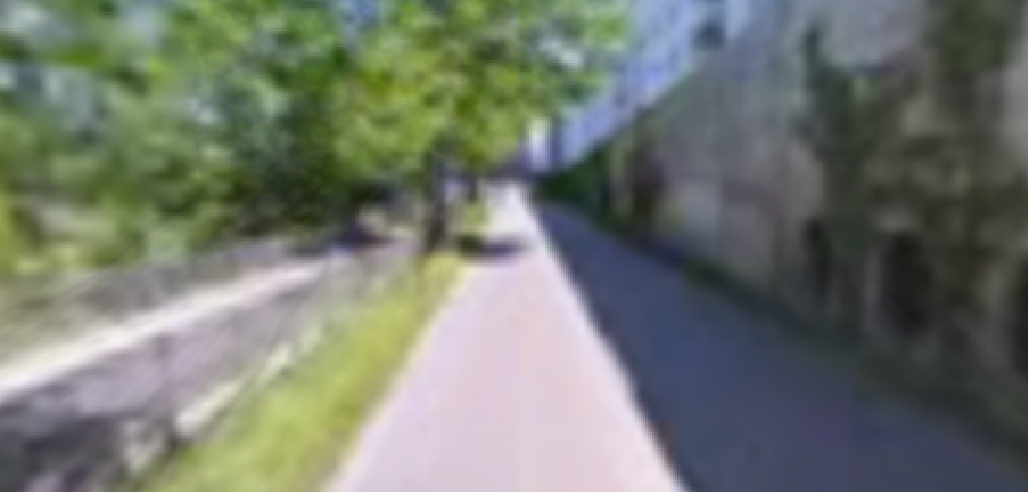
\includegraphics[width=1.0\linewidth]{src/screenshot_google_street_view_unscharf.png}
\caption{Verschwommene Interpolation von google Street View} % Titel der Grafik
\label{screenshot_google_street_view_unscharf} % Labelname
\end{figure}
Zudem wurden meist nur auf einer Fahrspur Fotos gemacht. Eine Ausnahme bilden die Autobahnen. Auf allen übrigen Strassen hat man sich darauf beschränkt Fotos nur in eine Richtung zu machen. Wenn man nun in die andere Richtung fahren möchte, sieht es so aus als würde man auf der falschen Seite fahren. Somit kommen einem die anderen Verkehrsteilnehmer, die sich ebenfalls auf den Fotos befinden, entgegen. Auch dieser Lösungsansatz muss deshalb verworfen werden. Eine weiter Möglichkeit besteht darin, dass eine eingene Umgebung entworfen wird.\\
Für den Fahrsimulator wird also eine virtuelle dreidimensionale Umgebung benötigt, in der man sich bewegen kann. Diese Umgebung, auch Szene genannt, setzt sich aus verschiedenen Objekten zusammen. Die Struktur eines solchen Objektes wird duch ein Mesh-File beschrieben. In einer Szene kann das gleiche Objekt mehrmals an verschiedenen Positionen vorkommen. Das Objekt kann durch eine Skalierung auch einmal gross und einmal klein erscheinen. Oder man variert sie mittels Rotatio. Zusätzlich wird mindestens ein Material-File benötigt, in dem sämtliche Texturen und Materialien, die von Objekten der Szene verwendet werden, definiert sind.
Ein Beispiel von einem Material, wie es in einem material-File definiert ist, wird im Listing \ref{example_materialfile_material} illustriert.
\begin{lstlisting}[caption={Beispiel aus dem material-File für ein Material},label={example_materialfile_material}]
material city_ground
{
	technique
	{
		pass
		{
			diffuse 0.0 0.0 0.0 1.00
			ambient 0.75 0.75 0.75 1.00	
		}
	}
}
\end{lstlisting}
Nach dem Keyword \textit{material} wird der Name des Materials angegeben. Als \textit{technique}-Block wird hier einer angegeben. Es können mehrere Blöcke angegeben werden. Diesen Blöcken können optional auch Namen gegeben werden, um zu erkennen wofür die einzelnen Blöcke sind. Ausgeführt wird jedoch immer nur einer der Blöcke, wobei der erste Block der Bevorzugteste und der unterste Block die letzte Fallbacklösung ist. Im \textit{pass}-Block werden die Reflektionswerte und die Farbe angegeben. Es können mehrere \textit{pass}-Blöcke angegeben werden, die jeweils hintereinander ausgeführt werden und sich überlagern. Das \textit{ambiant} als ambientes Licht bestimmt grundsätzlich die Farbe des Matierials. Die Zahlen representieren die RGB-Werte und können zwischen 0 und 1 liegen. Die Farbe des Materials in diesem Beispiel ist ein helles Grau. Die vierte Zahl representiert den Alphawert der Farbe. Der Alphawert quantifiziert die Sichtbarkeit des Materials wobei 1.0 voll sichtbar und 0.0 unsichtbar ist.
Weiter zeigt das Listing \ref{example_materialfile_texture} die definition einer Textur in einem material-File.\\
\newpage
\begin{lstlisting}[caption={Beispiel aus dem material-File zur Beschreibung einer Textur},label={example_materialfile_texture}]
material city_street_h
{
	technique
	{
		pass
		{
			diffuse 0.80 0.80 0.80 1.00

			texture_unit
			{
				texture street_h.png 2d 4
				filtering anisotropic
			}
		}
	}
}
\end{lstlisting}
Für die Textur wird in diesem Beispiel kein ambientes Licht definiert und es wird der Standartwert null genommen. Der diffuse Anteil bestimmt, wie stark das Material das Licht reflektiert. Da die Textur des Materials gut sichtbar sein soll, fällt dieser Wert relativ hoch aus. Im Block \textit{texture\_unit} wird die Textur angegeben und konfiguriert. Die Graphik, die als Textur verwendet wird, wird nach dem Keyword \textit{texture} angegeben. Das erste Argument nach der Graphikdatei, das \textit{2d}, konfiguriert die zweidimensionale Graphik als normale zweidimensionale Textur. Die vier als drittes Argument gibt die Anzahl zu generierenden Mipmaps an. Zusätzlich kann ein Filter für die Textur mit dem Keyword \textit{filtering} angegeben werden. Der anisotropische Filter wertet die Qualität der Textur in der Distanz auf. Hierbei wird die Richtung, der die Textur betrachtet wird, berücksichtigt.\\
Es werden zwei unterschiedliche Szenen für den Fahrsimulator erstellt. Die eine Szene zeigt eine Stadt mit Häusern, Kreuzungen und Verkehrsschildern. Die andere Szene stellt eine Berglandschaft mit mehreren Tunnels dar. Die Szenen werden mit dem Programm Cinema4D erstellt. 
\newpage
\subsubsection{Erstellen der Stadtszene}
\begin{figure}[H]
\centering 
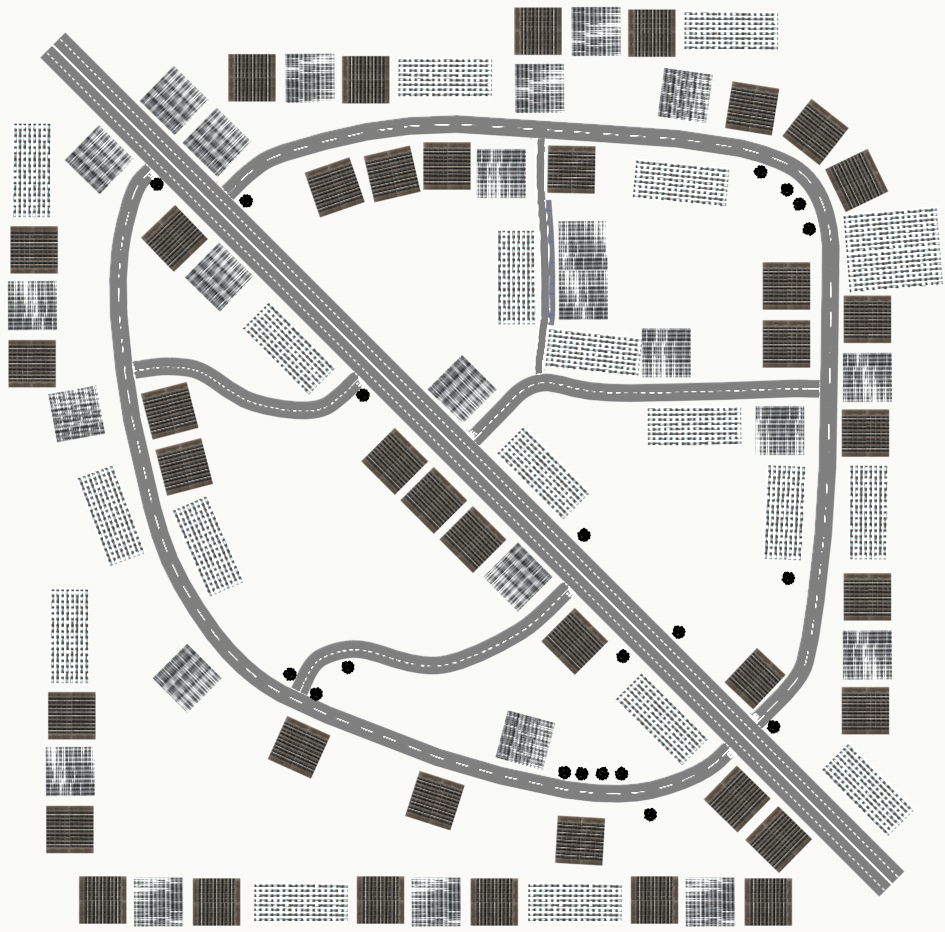
\includegraphics[width=1\linewidth]{src/CityWorld_map.png}
\caption{Karte der Stadtszene} % Titel der Grafik
\label{CityWorld_map} % Labelname
\end{figure}
Um die erstellte Stadtszene gut dokumentieren zu können, zeigt Abbildung \ref{CityWorld_map} eine Übersichtskarte. Die grosse vierspurige Strasse, die sich von oben links nach unten rechts durch die gesamte Szene zieht, ist eine rechteckige Ebene. Die Ebene ist mit einer Textur versehen, die die vier Spuren mit einer Sicherheitslinie in der Mitte darstellt. Die Länge der Textur entspricht jedoch nicht der Länge der Strasse. Wie in Abbildung \ref{examples_street_textures} zu sehen, entspricht die Textur nur einem kurzen Stück der Strasse. Die Textur wird auf der Ebene immer wiederholt. Auch bei allen anderen Strassen ist die Textur nur kurz und wird wiederholt.\\
\begin{figure}[H]
\centering 
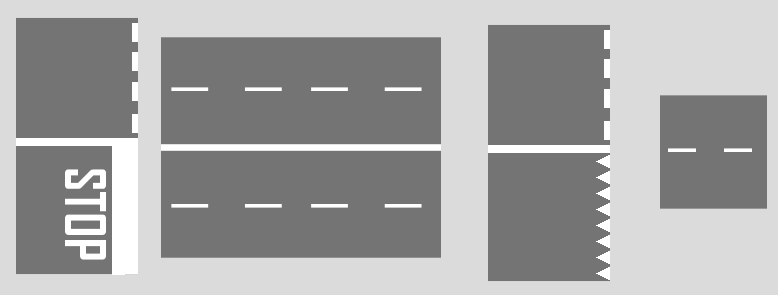
\includegraphics[scale=0.6]{src/examples_street_textures.png}
\caption{Beispiele von Strassentexturen} % Titel der Grafik
\label{examples_street_textures} % Labelname
\end{figure}
Die Strassen mit Kurven werden mit \glspl{spline} beschrieben. Eine Linie wird der \gls{spline} entlangeführt um die Breite einer Strasse zu erhalten. Die Textur der Strasse wird auf dieses, so zusammengefügte, Objekt gelegt. Der Abschluss solcher geschwungenen Strassen bilden wiederum rechteckige Ebenen. Diese erhalten die Textur einer Stoplinie mit Beschriftung auf der Strasse oder den vielen Dreieckigen Zeichen für kein Vortritt wie in Abbildung \ref{examples_street_textures} gezeigt. \\
Zusätzlich zu den Symbolen auf der Strasse, werden noch Verkehrsschilderobjekte in die Szene geladen. Die Abbildung \ref{screenshot_trafficsignal} zeigt ein Beipiel eines solchen Objektes. \\
\begin{figure}[H]
\centering 
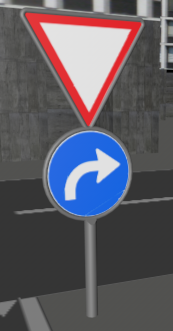
\includegraphics[scale=0.6]{src/screenshot_trafficsignal.png}
\caption{Beispiele eines Verkehrssignals} % Titel der Grafik
\label{screenshot_trafficsignal} % Labelname
\end{figure}

Die Häuser der Stadt sind einfache Blöcke, die mit dem Bild einer Hausfassade texturiert werden. Insgesammt sind drei Gebäudetypen, wie in Abbildung \ref{screenshot_buildings} dargestellt,  vorhanden. Diese drei Typen werden vervielfacht, eventuell gedreht und in der Szene verteilt.\\
Als nettes Extra wird das Hauptgebäude der ETH Zürich in die Szene eingefügt. Das Gebäudemodell stammt von Google 3D Warehouse und wird mit \gls{google-sketchup} bearbeitet. Dabei werden die Oberflächennormalen neu berechnet und die Bodenplatte, auf der das Gebäude steht, entfernt. Die Texturen werden manuell in das Material-File übernommen. Nun wird das ETH-Modell in die Szene geladen, skaliert und an der richtigen Stelle platziert. 

\begin{figure}[H]
\centering 
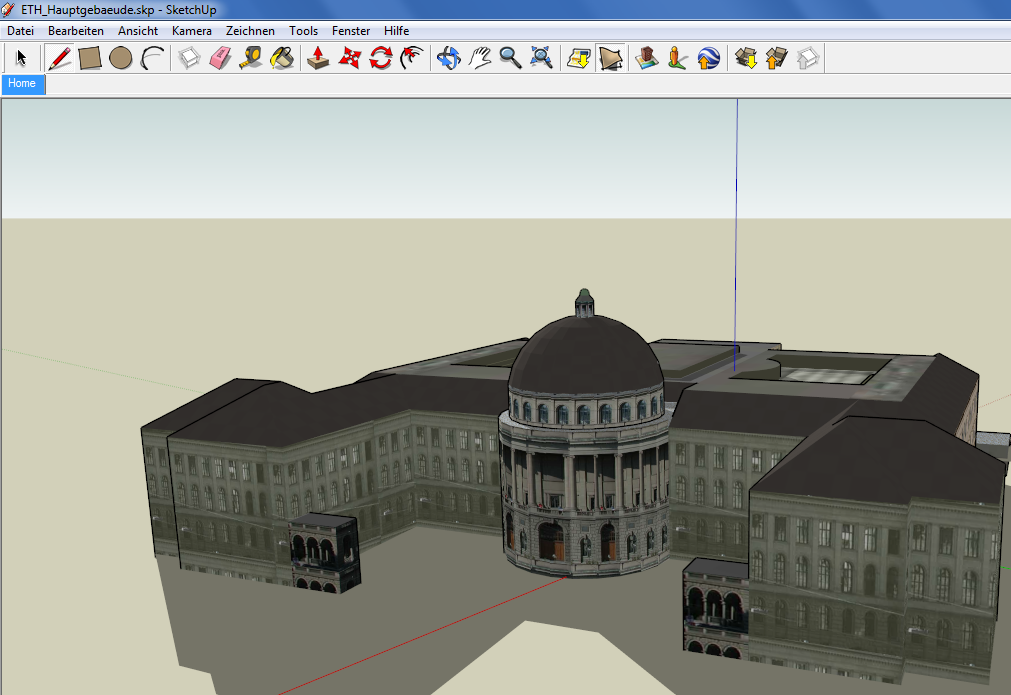
\includegraphics[width=1\linewidth]{src/screenshot_googlesketchup.png}
\caption{Das bearbeitete Modell der ETH Zürich} % Titel der Grafik
\label{googlesketchup_eth} % Labelname
\end{figure}

\begin{figure}[H]
\centering 
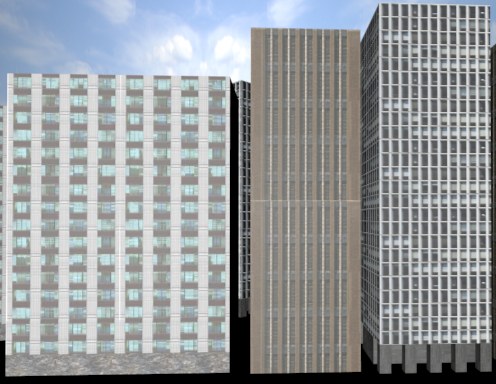
\includegraphics[scale=0.4]{src/screenshot_buildings.png}
\caption{Drei verschidene Gebäudetypen} % Titel der Grafik
\label{screenshot_buildings} % Labelname
\end{figure}
Um der Szene ein bisschen Farbe zu verleihen sind noch Bäume, wie in Abbildung \ref{screenshot_tree} in der Szene vorhanden. Ein Baum besteht aus einem Stamm mit einer Holztextur und einer Krone. Die Krone ist eine zufällig generierte Landschaft die zu einer Kugel geformt wird. Dadurch entstehen die verschiedenartigen Aus- und Einbuchtungen in der Baumkrone. Um die Illusion vollständig zu machen wird darauf eine Textur mit Blättern gelegt.\\

\begin{figure}[H]
\centering 
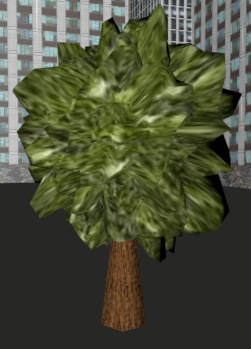
\includegraphics[scale=0.4]{src/screenshot_tree.png}
\caption{Baum} % Titel der Grafik
\label{screenshot_tree} % Labelname
\end{figure}

\subsubsection{Erstellung der Berglandschaft mit Tunnels}
Um die Berglandschaft zu generieren gibt es in Cinema4D ein eigens dafür vorgesehenes Objekt, das so genannte Landscape-Objekt. Durch die Konfiguration dieses Objekts kann die Gesamthöhe, sowie die Anzahl der Erhöhungen und Vertiefungen der Landschaft festgelegt werden. Mit einer Felstextur sieht dieses Objekt aus wie ein Berg.\\
Die Strasse in der Berglandschaft wird änlich der Strasse in der Stadtszene gemacht. Zusätzlich wird der \gls{spline} ein Quader entlanggezogen, welcher mit einer boolschen Operation vom Berg subtrahiert wird (Siehe Abbildung \ref{cinema4d_ausschneiden_tunnel}). Dadurch entsteht eine Röhre im Berg, welche aussieht wie ein Tunnel. Die Innenseite wird mit einer Betonplattenstruktur versehen.

\begin{figure}[H]
\centering 
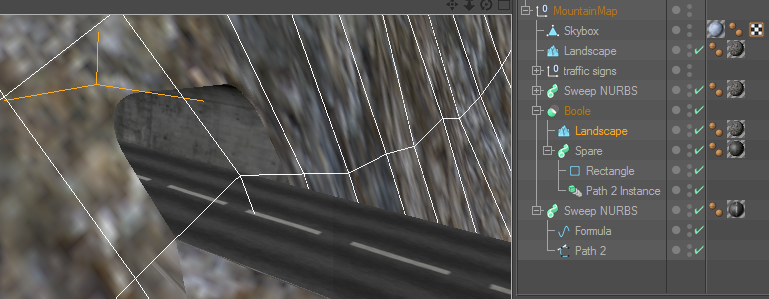
\includegraphics[width=1\linewidth]{src/screenshot_cinema4d.png}
\caption{Ausschneiden des Tunnels mit Cinema4D} % Titel der Grafik
\label{cinema4d_ausschneiden_tunnel} % Labelname
\end{figure}

\newpage
\subsubsection{Fahrzeug}
Zur Darstellung eines Autos wurde aus \gls{google-3d-warehouse} ein Mini Cooper heruntergeladen und in nach \gls{ogre-xml}konvertiert. Wie in Abbildung \ref{screenshot_minicooper} zu sehen, wird dieser aus der Perspektive einer dritten Person betrachtet. Beim Rückwärtsfahren wird die Kamera um das Fahrzeug gedreht, so dass man nach hinten sehen kann. Mit der Taste V auf der Tastatur kann die Ansicht in das innere des Fahrzeugs gewechselt werden. Zu Beginn wirde die Kamera lediglich in das innere des Mini Coopers versetzt, dorthin wo der Kopf des Fahrers in etwa sein sollte. In einem zweiten Schritt wurde jedoch eine eigene Fahrerkabine designed. Dies war vorallem deshalb notwendig, um eine Geschwindigkeitsanzeige implementieren zu können. 
\begin{figure}[H]
\centering 
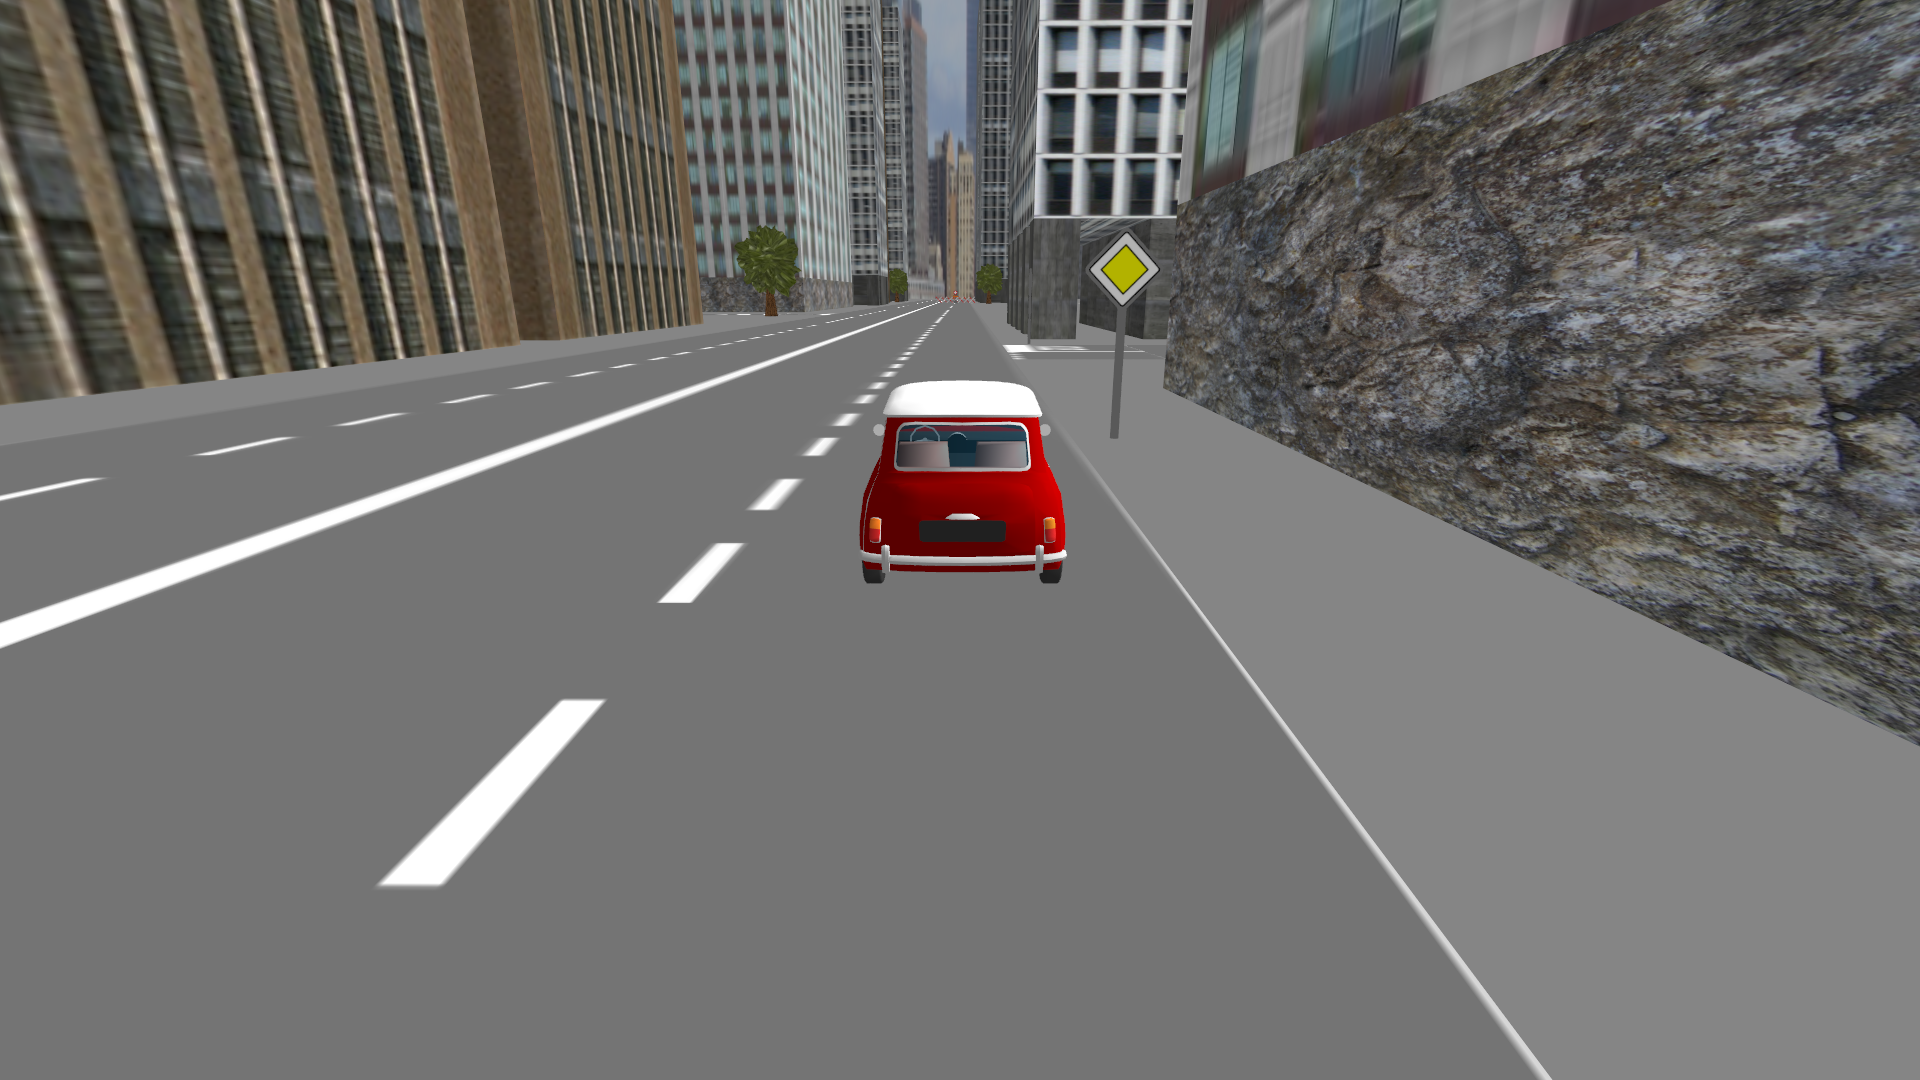
\includegraphics[width=1\linewidth]{src/screenshot_minicooper.png}
\caption{Der Mini Cooper aus der 3rd-Person-Ansicht} % Titel der Grafik
\label{screenshot_minicooper} % Labelname
\end{figure}

\newpage
\subsubsection{Fahrerkabine}
In der Innenansicht wird die Kamera so positioniert, dass der Benutzer die Szene aus dem Blickwinkel des Fahrzeugführers wahrnimmt. Dazu wird das Fahrzeug ausgeblendet und ein Modell wird sichtbar. Dieses besteht aus drei getrennten Objekten:
\begin{itemize}
	\item dem Cockpit, bestehend aus dem Armaturenbrett, der linken \gls{a-saeule} und dem Dach
	\item dem Tachozeiger, welcher relativ zum Cockpit positioniert und entsprechend der aktuellen Geschwindigkeit gedreht wird.
	\item dem Steuerrad, welches auch relativ zum Cockpit positioniert und entsprechend dem Lenkeinschlag rotiert wird.
\end{itemize}

\begin{figure}[H]
\centering 
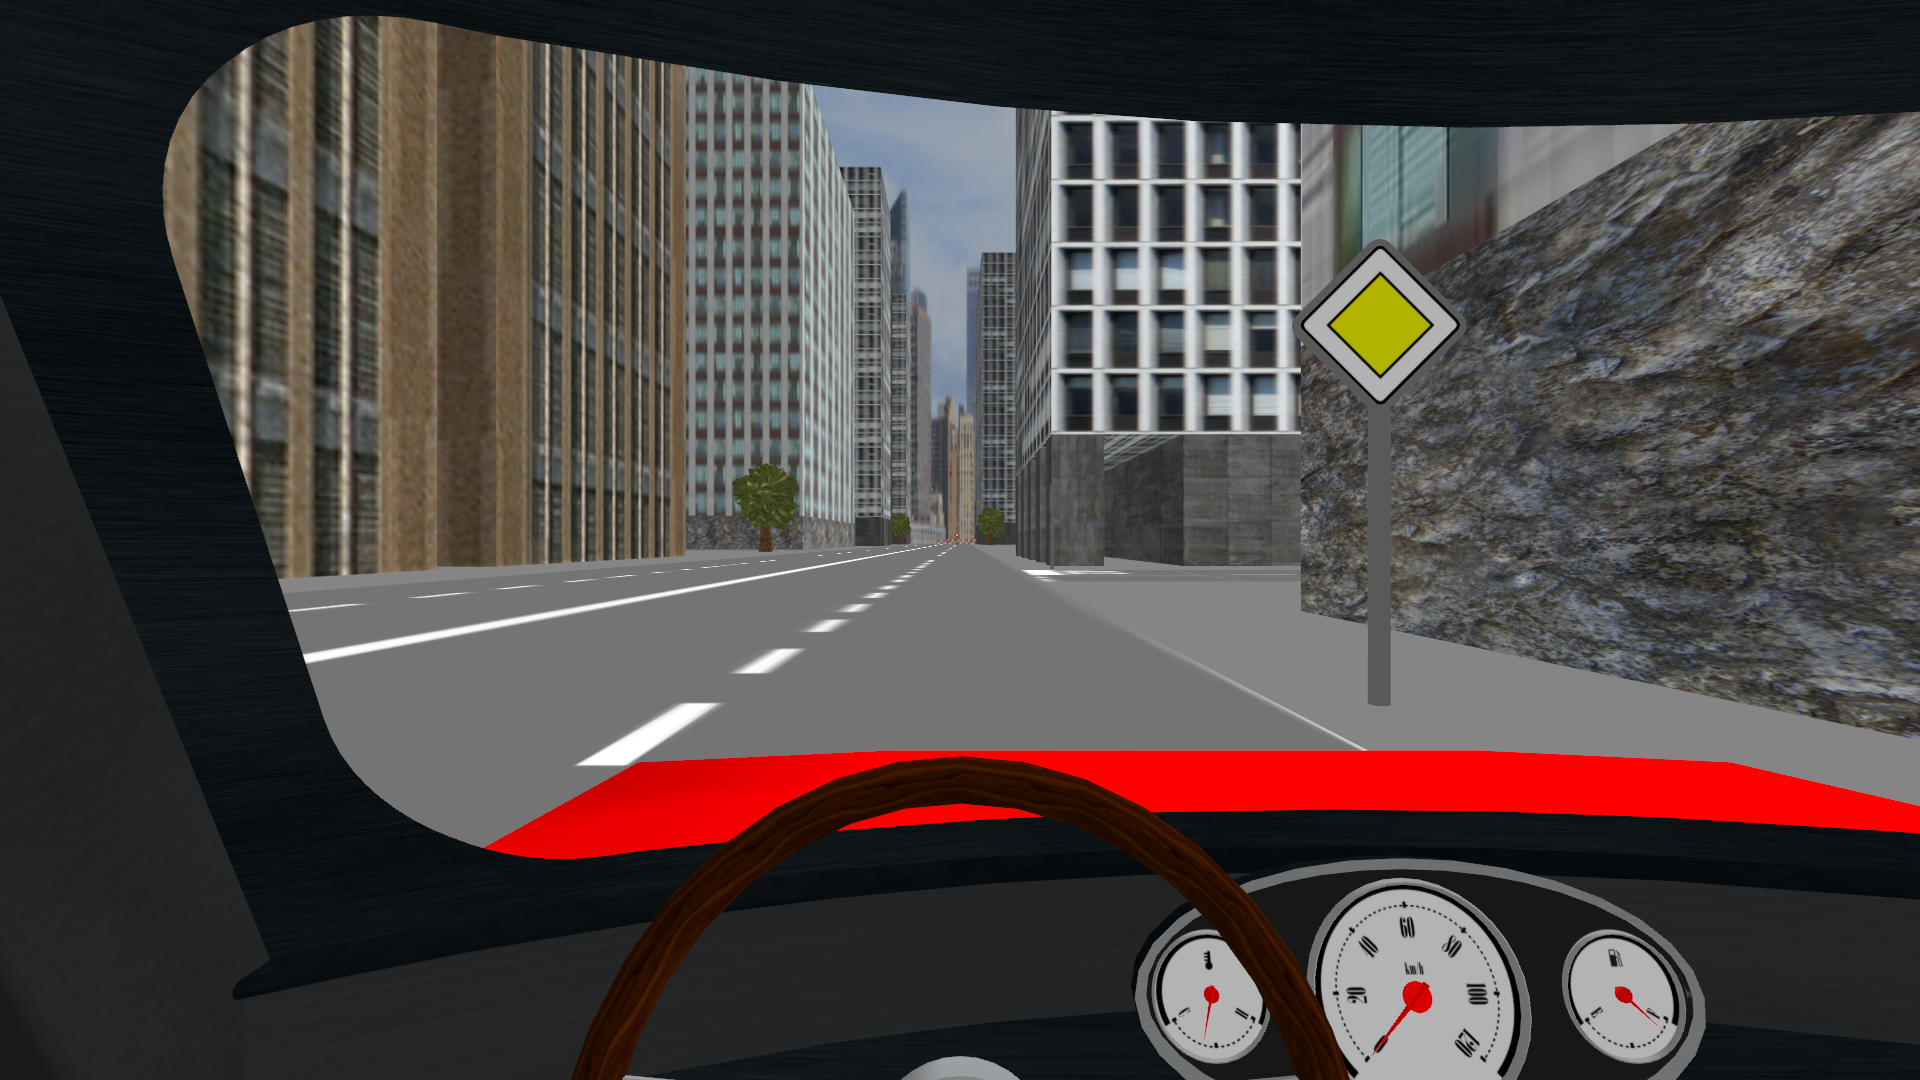
\includegraphics[width=1\linewidth]{src/screenshot_cockpit.png}
\caption{Innenansicht des Mini} % Titel der Grafik
\label{screenshot_cockpit} % Labelname
\end{figure}
Um die Geschwindigkeit des Fahrzeuges herauszufinden, wird die Skalierung aller Objekte so gewählt, dass im Cinema4D mit reellen Werten gearbeitet werden konnte. So sind die Strassenspuren drei Meter breit modeliert. Um die Geschwindigkeit zu ermitteln, wurde in Cinema4D eine Distanz abgemessen und diese mit verschiedenen Konstanten Geschwindigkeiten abgefahren und die Zeit gemessen. Die interne Geschwindigkeit im Programm wird mit einem Faktor in die tatsächliche Geschwindigkeit umgerechnet. Diese kann dann auf dem Tachometer angezeigt werden.\\
\begin{figure}[H]
\centering 
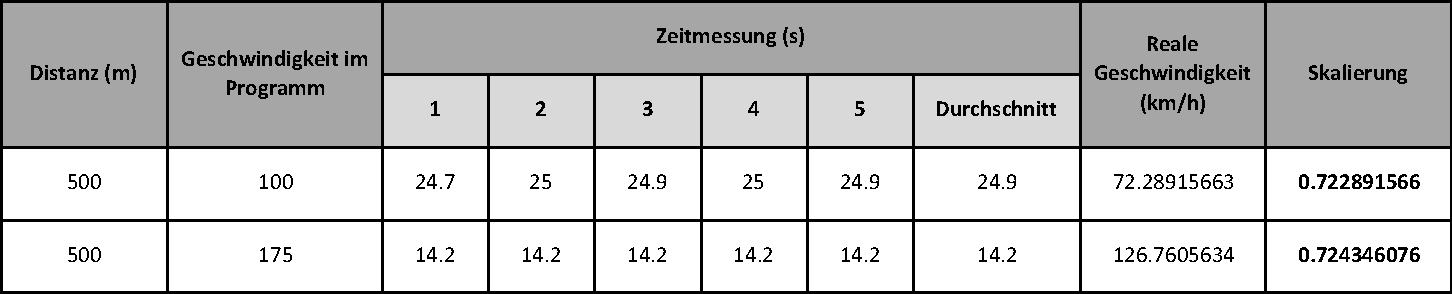
\includegraphics[width=1\linewidth]{src/geschwindigkeitsberechnung.pdf}
\caption{Berechnung der tatsächlichen Geschwindigkeit} % Titel der Grafik
\label{berechnung_geschwindigkeit} % Labelname
\end{figure}

\newpage
\subsection{Hautpprogramm}

%Sequenzdiagramm
%Blockdiagramm

\begin{figure}[H]
\centering 
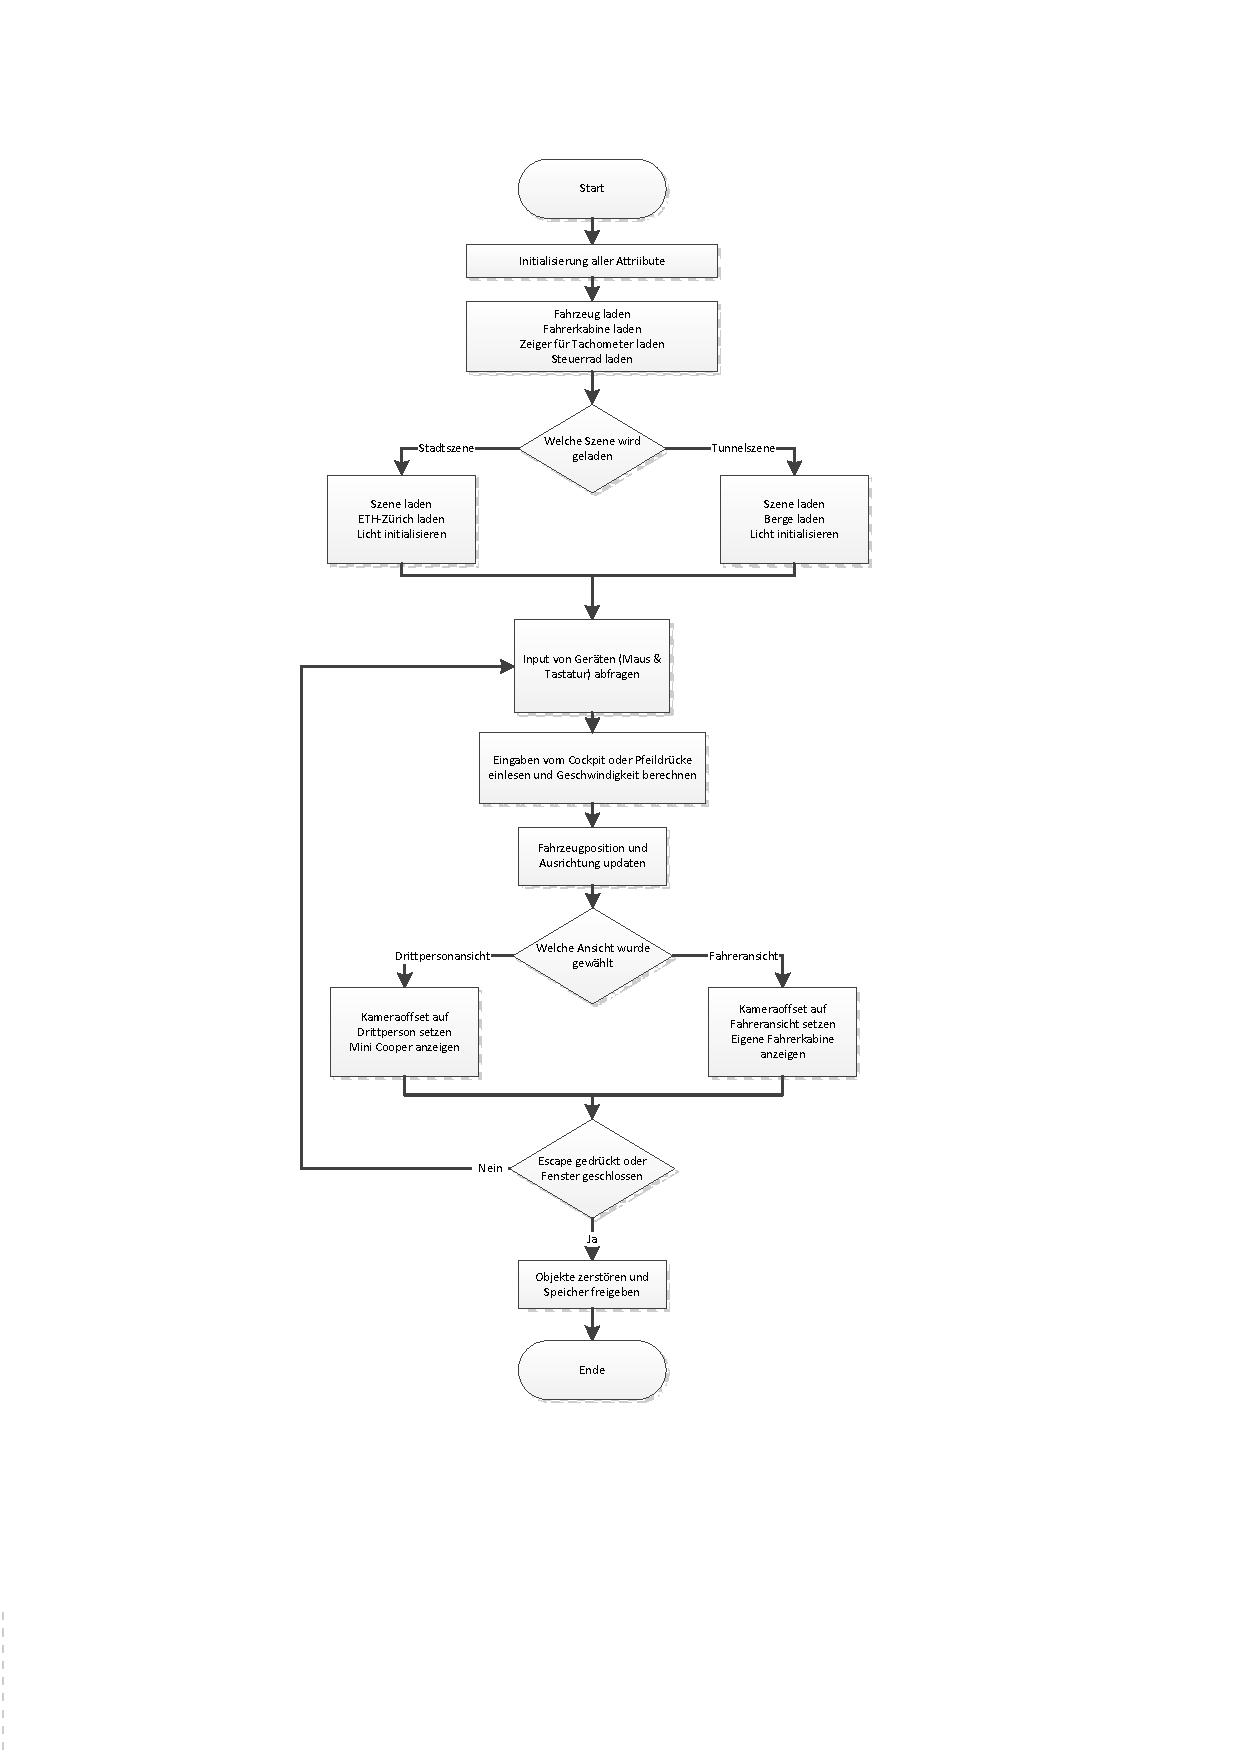
\includegraphics[width=0.6\linewidth]{src/flowchart_mainapplication.pdf}
\caption{Ablauf des Hauptprogramms} % Titel der Grafik
\label{ablauf_hauptprogramm} % Labelname
\end{figure}

\newpage

\subsubsection{Initialisierung}

Beim Start der Applikation werden die Konfigurationsfiles (siehe Kapitel \ref{sec:konfigurationsfiles}) geladen. Aus den darin enthaltenen Informationen wird das Grundgerüst von OGRE erstellt. Dazu gehören folgende Objekte:

\minisec{rootNode}
Der RootNode der 3D-Szene. Alle Objekte sind diesem angehängt.
\minisec{renderWindow}
Das RenderWindow ist das sichtbare Fenster der Applikation. In ihm wird der gesamte grafische Inhalt dargestellt.
\minisec{camera}
Wie der Name vermuten lässt, ist dies die Kamera, durch welche der Benutzer die Szene beobachtet.
\minisec{viewPort}
Der ViewPort ist mit dem Kameraobjekt verknüpft und zeigt die Bildprojektion der 3D-Szene an. 

\begin{lstlisting}[caption={Laden der Konfigurationsdateien},label={laden_konfigurationsdateien}]
// create root node
#ifdef _DEBUG
rootNode = new Ogre::Root("Resources/plugins_d.cfg", "Resources/graphics_d.cfg", "log_d.txt");
#else
rootNode = new Ogre::Root("Resources/plugins.cfg", "Resources/graphics.cfg", "log.txt");
#endif

// load config file
Ogre::ConfigFile configFile;
#ifdef _DEBUG
configFile.load("Resources/resources_d.cfg");
#else
configFile.load("Resources/resources.cfg");
#endif

// load resource files
Ogre::ConfigFile::SectionIterator it = configFile.getSectionIterator();
while(it.hasMoreElements())
{
	Ogre::String sectionName = it.peekNextKey();
	Ogre::ConfigFile::SettingsMultiMap* settings = it.getNext();
	Ogre::ConfigFile::SettingsMultiMap::iterator i;
	for(i = settings->begin(); i != settings->end(); ++i)
	{
		Ogre::ResourceGroupManager::getSingleton(). addResourceLocation(i->second, i->first, sectionName);
	}
}

// try to initialize window with settings from config file
if(!(rootNode->restoreConfig()))
{
	throw Ogre::Exception(Ogre::Exception::ERR_INVALID_STATE, "Could not read graphics configuration", "MainApplication::go");
}

renderWindow = rootNode->initialise(true, "Driving Simulator V1");

// initialize resources
Ogre::TextureManager::getSingleton().setDefaultNumMipmaps(5);
Ogre::ResourceGroupManager::getSingleton(). initialiseAllResourceGroups();

// create scene manager
sceneManager = rootNode->createSceneManager("DefaultSceneManager");

// create camera
camera = sceneManager->createCamera("PlayerCam");
camera->setAutoAspectRatio(true);
camera->setNearClipDistance(1);

// add viewport
Ogre::Viewport* viewPort = renderWindow->addViewport(camera);
viewPort->setBackgroundColour(Ogre::ColourValue(0, 0, 0));
\end{lstlisting}

\subsubsection{Konfigurationsfiles}
\label{sec:konfigurationsfiles}

Die Applikation verwendet folgende Dateien zur Konfiguration beim Start:

\minisec{plugins.cfg}
\gls{ogre} lädt einige Komponente, die zur Ausführung des Programms benötigt werden, zur Laufzeit. Welche Komponenten geladen werden, wird im File plugins.cfg definiert. Inhalt siehe Anhang \ref{listing:plugins.cfg}.

\minisec{graphics.cfg}
In diesem File sind die Grafikeinstellungen definiert. Inhalt siehe Anhang \ref{listing:graphics.cfg}.

\minisec{resources.cfg}
Hier werden alle Pfade angegeben, in welchen sich benötigte Resourcen (z.B. Mesh-Files, Bilder, etc.) befinden. Inhalt siehe Angang \ref{listing:resources.cfg}.

\subsubsection{Laden des Autos}

\begin{lstlisting}[caption={Laden des Autos},label={laden_auto}]
void DrivingSimulatorV1::createCar()
{
	// load car
	Ogre::Entity* car = sceneManager->createEntity("MiniCooper.mesh");
	carNode = sceneManager->getRootSceneNode()->createChildSceneNode();
	carNode->attachObject(car);
	carNode->scale(4, 4, 4);

	// load Cockpit
	Ogre::Entity* cockpit = sceneManager->createEntity("MiniCockpit.mesh");
	cockpitNode = sceneManager->getRootSceneNode()->createChildSceneNode();
	cockpitNode->attachObject(cockpit);
	cockpitNode->scale(0.05, 0.05, 0.05);

	Ogre::Entity* pointer = sceneManager->createEntity("MiniCockpitPointer.mesh");
	pointerNode = sceneManager->getRootSceneNode()->createChildSceneNode();
	pointerNode->attachObject(pointer);
	pointerNode->scale(0.02, 0.02, 0.02);

	Ogre::Entity* steeringWheel = sceneManager->createEntity("MiniCockpitSteeringWheel.mesh");
	steeringWheelNode = sceneManager->getRootSceneNode()->createChildSceneNode();
	steeringWheelNode->attachObject(steeringWheel);
	steeringWheelNode->scale(0.03, 0.03, 0.03);

	// setup camera
	camera->setFOVy(Ogre::Degree(70));
}
\end{lstlisting}

Hier werden die drei Modelle \textit{MiniCooper.mesh}, \textit{MiniCockpitPointer.mesh} und \textit{MiniSteeringWheel.mesh} durch den Szenenmanager geladen und jeweils einem eigenen \gls{node} angehängt und entsprechend skaliert, so dass sie in die Szene passen.

\subsubsection{Laden des Szene}

\begin{lstlisting}[caption={Laden der Szene},label={laden_szene}]
void DrivingSimulatorV1::createScene1() // city
{
	// create world node
	Ogre::SceneNode* worldNode = sceneManager->getRootSceneNode()->createChildSceneNode();
	Ogre::Entity* cityWorld = sceneManager->createEntity("CityWorld.mesh");
	worldNode->scale(0.05, 0.05, 0.05);
	worldNode->attachObject(cityWorld);

	// create ETH Node
	Ogre::SceneNode* ethNode = sceneManager->getRootSceneNode()->createChildSceneNode();
	Ogre::Entity* eth = sceneManager->createEntity("ETH.mesh");
	ethNode->attachObject(eth);
	ethNode->scale(1.3, 1.3, 1.3);
	ethNode->setPosition(428, 0, 235);
	ethNode->yaw(Ogre::Degree(210));

	// create ambient light
	sceneManager->setAmbientLight(Ogre::ColourValue(0.7, 0.7, 0.7));

	// create sun light
	Ogre::Light* sunLight = sceneManager->createLight();
	sunLight->setType(Ogre::Light::LT_DIRECTIONAL);
	sunLight->setDirection(Ogre::Vector3(-0.5, -0.5, 0.5));
	sunLight->setDiffuseColour(Ogre::ColourValue(1, 1, 1));
	sunLight->setSpecularColour(Ogre::ColourValue(0.7, 0.7, 0.7));

	// set car to initial position and orientation
	carNode->setPosition(584, 0, 121);
	carNode->setOrientation(Ogre::Quaternion(Ogre::Degree(-4.5), Ogre::Vector3::UNIT_Y));
}
\end{lstlisting}

Ähnlich zur Funktion \textit{createCar} (Abschnitt \ref{laden_auto}) werden hier zunächst Objekte geladen. Diesmal die beiden Meshes \textit{CityWorld.mesh} und \textit{ETH.mesh}. Auch sie werden jeweils eigenen Nodes angehängt und entsprechend positioniert, ausgerichtet und skaliert. Weiter wird in dieser Funktion die Belichtung der Szene definiert. Einmal wird mit \textit{setAmbientLight} das Umgebungslicht gesetzt, danach wird eine neue direktionale Lichtquelle erstellt, die in unserem Programm das Sonnenlicht liefert. Zuletzt wird das Auto an die korrekte Startposition in der Szene gesetzt und ausgerichtet.\\Das Laden der Tunnelszene geschieht in der Funktion \textit{createScene2}. Details dazu im Listing \textit{DrivingSimulatorV1.cpp} auf der beiliegenden CD.

\subsubsection{Callback-Methode}

Die so genannte \gls{callback-methode} wird durch einen internen Timer des \gls{ogre}-Frameworks aufgerufen. Dies geschieht je nach \gls{vsync}-Konfiguration entweder mit der Bildwiederholungsrate der Bildschirms z.B. 60 mal pro Sekunde oder so oft wie möglich. Über die Variable timeSinceLastFrame ist genau bestimmt, wie lange der letzte Renderdurchlauf zurück liegt. Die Aufgabe dieser Methode ist alles das zu tun, was vor dem Zeichnen eines neuen Bildes getan werden muss. Dazu gehört folgendes:

\subsubsection*{Tastatur- und Mauseingaben abfragen}
\begin{lstlisting}[caption={Abfragen der Eingabegeräte},label={abfragen_eingabe_geraete}]
// capture input devices
if(inputManager)
{
	keyboard->capture();
	mouse->capture();
}
\end{lstlisting}

\subsubsection*{Geschwindigkeit reduzieren}
\begin{lstlisting}[caption={Geschwindigkeit reduzieren},label={geschwindigkeit_reduzieren}]
// decrease speed (air resistance, etc...)
if(speed > 0)
	speed *= Ogre::Math::Pow(0.92, evt.timeSinceLastFrame);
else
	speed *= Ogre::Math::Pow(0.7, evt.timeSinceLastFrame);
\end{lstlisting}
Gibt man kein Gas, so verlangsamt sich das Fahrzeug durch das Einwirken diverser Kräfte (z.B. Luft- und Rollwiderstand, Rebungskräfte innerhalb von Motor und Getriebe, etc.). Dies wird durch das Multiplizieren mit einem Wert kleiner 1 simuliert. Da nicht immer bekannt ist, wie oft diese Methode pro Sekunde ausgeführt wird, potenziert man diesen Wert mit der Anzahl vergangener Sekunden seit dem letzten Renderdurchlauf. So ist definiert, dass sich die Geschwindigkeit des Autos pro Sekunde um den Faktor 0.92 bzw. 0.7 verringert.

\subsubsection*{Beschleunigen oder Bremsen}
\begin{lstlisting}[caption={Beschleunigen oder Bremsen},label={beschleunigen_oder_bremsen}]
// udp input
if(UdpListener::throttle >= 0)
	speed += UdpListener::throttle * 9 * evt.timeSinceLastFrame;
else
	speed += UdpListener::throttle * 30 * evt.timeSinceLastFrame;

// keyboard input
if(keyboard->isKeyDown(OIS::KC_UP))
	speed += 9 * evt.timeSinceLastFrame;
if(keyboard->isKeyDown(OIS::KC_DOWN))
	speed -= 30 * evt.timeSinceLastFrame;
\end{lstlisting}
Abhängig vom Ausschlag des Gas- bzw. Bremspedals wird das Fahrzeug beschleunigt oder abgebremst. Auch hier wird die \textit{timeSinceLastFrame}-Variable verwendet um das zeitliche Verhalten genau zu definieren. Das Drücken der \textit{Pfeil-oben}-Taste entspricht dem vollständig durchgedrückten Gaspedal. Analog dazu löst das Drücken der \textit{Pfeil-unten}-Taste eine Vollbremsung aus.

\subsubsection*{Fahrzeug lenken}
\begin{lstlisting}[caption={Fahrzeug lenken},label={fahrzeug_lenken}]
// calculate steer intensity
Ogre::Real normalizedSpeed = Ogre::Math::Abs(speed / 180);
Ogre::Real steerIntensity = 100 / (100 * (Ogre::Math::Pow(normalizedSpeed, 2)) + 1) * Ogre::Math::Pow(normalizedSpeed, 1.5);

// rotate car by udp input
carNode->yaw(Ogre::Degree(UdpListener::steer * -5 * evt.timeSinceLastFrame * speed));
cameraRotationOffset += UdpListener::steer * 90 * evt.timeSinceLastFrame;

// rotate car by keyboard input
if(keyboard->isKeyDown(OIS::KC_LEFT))
	keyboardSteer += 270 * evt.timeSinceLastFrame;
if(keyboard->isKeyDown(OIS::KC_RIGHT))
	keyboardSteer -= 270 * evt.timeSinceLastFrame;
\end{lstlisting}
Wenn das Fahrzeug in eine Richtung gelenkt werden soll, findet eine Rotation um die Y-Achse statt. Die Geschwindigkeit, mit der rotiert wird (hier \textit{steerIntensity}), ist von der Geschwindigkeit des Fahrzeugs abhängig und wird hier von einer nicht-linearen Funktion beschrieben. Damit soll das \gls{untersteuern} des Fahrzeugs bei hochen Geschwindigkeiten simuliert werden.

\begin{figure}[H]
\centering 
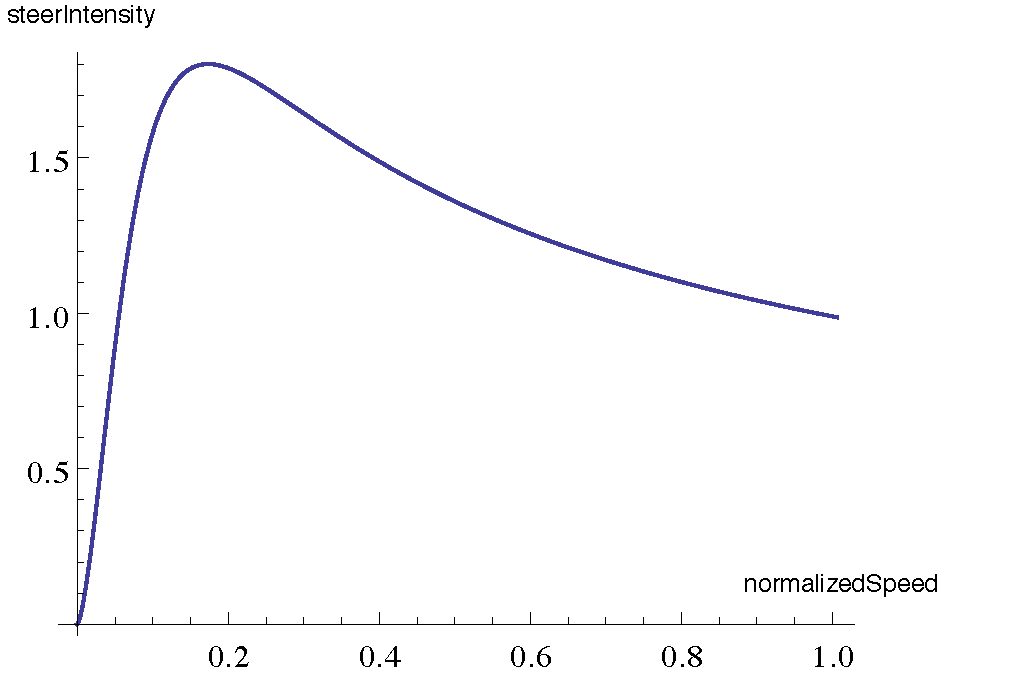
\includegraphics[width=0.7\linewidth]{src/steerIntensity.pdf}
\caption{Steuerintensität in Abhängigkeit der Geschwindigkeit} % Titel der Grafik
\label{steer_intensity} % Labelname
\end{figure}

\subsubsection*{Fahrzeug bewegen}
\begin{lstlisting}[caption={Fahrzeug bewegen},label={fahrzeug_bewegen}]
// update car position
Ogre::Real xMove = Ogre::Math::Sin(carNode->getOrientation().getYaw()) * speed * evt.timeSinceLastFrame;
Ogre::Real zMove = Ogre::Math::Cos(carNode->getOrientation().getYaw()) * speed * evt.timeSinceLastFrame;
carNode->translate(xMove, 0, zMove);
\end{lstlisting}

Die Koordinaten des Autos werden ensprechend seiner Ausrichtung und Geschwindigkeit neu berechnet.

\subsubsection*{Kamera positionieren}
\begin{lstlisting}[caption={Positionierung der 1st-Person-Kamera},label={positionierung_fp_kamera}]
// position camera
Ogre::Vector3 cameraOffset(1.3, 4.0, 0.7);
camera->setOrientation(carNode->getOrientation() * Ogre::Quaternion(Ogre::Degree(180), Ogre::Vector3::UNIT_Y));
camera->setPosition(carNode->getPosition() + carNode->getOrientation() * cameraOffset);
\end{lstlisting}
In der \gls{1st-person}-Ansicht wird die Kamera an die Stelle, an der sich der Kopf des Fahrers befindet verschoben.\\

\begin{lstlisting}[caption={Positionierung der 3rd-Person-Kamera},label={positionierung_tp_kamera}]
if(gear != REVERSE)
	cameraRotationOffset *= Ogre::Math::Pow(0.1, evt.timeSinceLastFrame);
else
	cameraRotationOffset = cameraRotationOffset * Ogre::Math::Pow(0.1, evt.timeSinceLastFrame) + 180 * (1 - Ogre::Math::Pow(0.1, evt.timeSinceLastFrame));

Ogre::Radian camAngle = carNode->getOrientation().getYaw() + Ogre::Degree(cameraRotationOffset);
Ogre::Real camXOffset = -Ogre::Math::Sin(camAngle) * 25;
Ogre::Real camYOffset = 8;
Ogre::Real camZOffset = -Ogre::Math::Cos(camAngle) * 25;

camera->setPosition(carNode->getPosition() + Ogre::Vector3(camXOffset, camYOffset, camZOffset));
camera->lookAt(carNode->getPosition());

carNode->setVisible(true);
cockpitNode->setVisible(false);
pointerNode->setVisible(false);
steeringWheelNode->setVisible(false);
\end{lstlisting}

Im \gls{3rd-person}-Modus wird die Kamera um eine bestimmte Distanz nach hinten verschoben und zum Mittelpunkt des Fahrzeugs ausgerichtet.



